\section{dg::Polygonizer Class Reference}
\label{classdg_1_1Polygonizer}\index{dg::Polygonizer@{dg::Polygonizer}}
{\tt \#include $<$Polygonizer.h$>$}

Collaboration diagram for dg::Polygonizer:\begin{figure}[H]
\begin{center}
\leavevmode
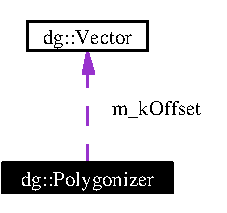
\includegraphics[width=72pt]{classdg_1_1Polygonizer__coll__graph}
\end{center}
\end{figure}
\subsection*{Public Types}
\begin{CompactItemize}
\item 
typedef {\bf Set}$<$ {\bf Color} $>$ {\bf Color\-List}
\item 
typedef {\bf Set}$<$ {\bf Vector} $>$ {\bf Vector\-List}
\item 
typedef {\bf Real}($\ast$ {\bf Function} )({\bf Real} f\-X, {\bf Real} f\-Y, {\bf Real} f\-Z)
\item 
enum {\bf March\-Method} \{ {\bf MM\_\-CUBES}, 
{\bf MM\_\-TETRA}
 \}
\end{CompactItemize}
\subsection*{Public Methods}
\begin{CompactItemize}
\item 
{\bf Polygonizer} ({\bf Function} pv\-Function=NULL, {\bf Int} i\-Cell\-Count=8, {\bf Real} f\-Scale=1.0, {\bf Real} f\-Iso\-Level=1.0)
\item 
{\bf Real} {\bf sample} ({\bf Real} f\-X, {\bf Real} f\-Y, {\bf Real} f\-Z)
\item 
void {\bf set\-Function} ({\bf Function} pv\-Function)
\item 
void {\bf set\-Inverse\-Normals} (bool b\-Inv\-Normals)
\item 
bool {\bf get\-Inverse\-Normals} ()
\item 
void {\bf set\-Cell\-Count} ({\bf Int} i\-Cell\-Count)
\item 
{\bf Int} {\bf get\-Cell\-Count} ()
\item 
void {\bf set\-Iso\-Level} ({\bf Real} f\-Iso\-Level)
\item 
{\bf Real} {\bf get\-Iso\-Level} ()
\item 
void {\bf set\-Offset} ({\bf Real} f\-X, {\bf Real} f\-Y, {\bf Real} f\-Z)
\item 
void {\bf get\-Offset} ({\bf Real} \&f\-X, {\bf Real} \&f\-Y, {\bf Real} \&f\-Z)
\item 
void {\bf set\-Scale} ({\bf Real} f\-Scale)
\item 
{\bf Real} {\bf get\-Scale} ()
\item 
void {\bf set\-Epsilon} ({\bf Real} f\-Epsilon)
\item 
{\bf Real} {\bf get\-Epsilon} ()
\item 
{\bf Vector\-List} \& {\bf get\-Vertices} ()
\item 
{\bf Vector\-List} \& {\bf get\-Normals} ()
\item 
{\bf Color\-List} \& {\bf get\-Colors} ()
\item 
{\bf Real} {\bf get\-Intersect} ({\bf Real} f\-V1, {\bf Real} f\-V2, {\bf Real} f\-Level)
\item 
void {\bf get\-Color} ({\bf Color} \&rk\-Color, {\bf Vector} \&rk\-Pos, {\bf Vector} \&rk\-Normal)
\item 
void {\bf get\-Normal} ({\bf Vector} \&rk\-Normal, {\bf Real} f\-X, {\bf Real} f\-Y, {\bf Real} f\-Z)
\item 
void {\bf march\-Cube} ({\bf Real} f\-X, {\bf Real} f\-Y, {\bf Real} f\-Z, {\bf Real} f\-Scale)
\item 
void {\bf march\-Tetra} ({\bf Vector} $\ast$pak\-Tetra\-Pos, {\bf Real} $\ast$paf\-Tetra\-Value)
\item 
void {\bf march\-Tetra\-Cube} ({\bf Real} f\-X, {\bf Real} f\-Y, {\bf Real} f\-Z, {\bf Real} f\-Scale)
\item 
void {\bf evaluate} ({\bf March\-Method} e\-Type=MM\_\-TETRA)
\end{CompactItemize}
\subsection*{Protected Attributes}
\begin{CompactItemize}
\item 
{\bf Function} {\bf m\_\-pv\-Function}
\item 
bool {\bf m\_\-b\-Inverse\-Normals}
\item 
{\bf Int} {\bf m\_\-i\-Cell\-Count}
\item 
{\bf Real} {\bf m\_\-f\-Scale}
\item 
{\bf Real} {\bf m\_\-f\-Delta}
\item 
{\bf Real} {\bf m\_\-f\-Epsilon}
\item 
{\bf Real} {\bf m\_\-f\-Iso\-Level}
\item 
{\bf Vector} {\bf m\_\-k\-Offset}
\item 
{\bf Vector\-List} {\bf m\_\-k\-Vertex\-List}
\item 
{\bf Vector\-List} {\bf m\_\-k\-Normal\-List}
\item 
{\bf Color\-List} {\bf m\_\-k\-Color\-List}
\end{CompactItemize}


\subsection{Member Typedef Documentation}
\index{dg::Polygonizer@{dg::Polygonizer}!ColorList@{ColorList}}
\index{ColorList@{ColorList}!dg::Polygonizer@{dg::Polygonizer}}
\subsubsection{\setlength{\rightskip}{0pt plus 5cm}typedef {\bf Set}$<${\bf Color}$>$ dg::Polygonizer::Color\-List}\label{classdg_1_1Polygonizer_s0}




Definition at line 26 of file Polygonizer.h.\index{dg::Polygonizer@{dg::Polygonizer}!Function@{Function}}
\index{Function@{Function}!dg::Polygonizer@{dg::Polygonizer}}
\subsubsection{\setlength{\rightskip}{0pt plus 5cm}typedef {\bf Real}($\ast$ dg::Polygonizer::Function)({\bf Real} f\-X, {\bf Real} f\-Y, {\bf Real} f\-Z)}\label{classdg_1_1Polygonizer_s2}




Definition at line 28 of file Polygonizer.h.\index{dg::Polygonizer@{dg::Polygonizer}!VectorList@{VectorList}}
\index{VectorList@{VectorList}!dg::Polygonizer@{dg::Polygonizer}}
\subsubsection{\setlength{\rightskip}{0pt plus 5cm}typedef {\bf Set}$<${\bf Vector}$>$ dg::Polygonizer::Vector\-List}\label{classdg_1_1Polygonizer_s1}




Definition at line 27 of file Polygonizer.h.

\subsection{Member Enumeration Documentation}
\index{dg::Polygonizer@{dg::Polygonizer}!MarchMethod@{MarchMethod}}
\index{MarchMethod@{MarchMethod}!dg::Polygonizer@{dg::Polygonizer}}
\subsubsection{\setlength{\rightskip}{0pt plus 5cm}enum dg::Polygonizer::March\-Method}\label{classdg_1_1Polygonizer_s5}


\begin{Desc}
\item[Enumeration values: ]\par
\begin{description}
\index{MM_CUBES@{MM\_\-CUBES}!dg::Polygonizer@{dg::Polygonizer}}\index{dg::Polygonizer@{dg::Polygonizer}!MM_CUBES@{MM\_\-CUBES}}\item[{\em 
{\em MM\_\-CUBES}\label{classdg_1_1Polygonizer_s5s3}
}]\index{MM_TETRA@{MM\_\-TETRA}!dg::Polygonizer@{dg::Polygonizer}}\index{dg::Polygonizer@{dg::Polygonizer}!MM_TETRA@{MM\_\-TETRA}}\item[{\em 
{\em MM\_\-TETRA}\label{classdg_1_1Polygonizer_s5s4}
}]\end{description}
\end{Desc}



Definition at line 19 of file Polygonizer.h.

\subsection{Constructor \& Destructor Documentation}
\index{dg::Polygonizer@{dg::Polygonizer}!Polygonizer@{Polygonizer}}
\index{Polygonizer@{Polygonizer}!dg::Polygonizer@{dg::Polygonizer}}
\subsubsection{\setlength{\rightskip}{0pt plus 5cm}Polygonizer::Polygonizer ({\bf Function} {\em pv\-Function} = NULL, {\bf Int} {\em i\-Cell\-Count} = 8, {\bf Real} {\em f\-Scale} = 1.0, {\bf Real} {\em f\-Iso\-Level} = 1.0)}\label{classdg_1_1Polygonizer_a0}




Definition at line 8 of file Polygonizer.cpp.

References dg::Int, m\_\-f\-Delta, m\_\-f\-Epsilon, m\_\-f\-Iso\-Level, m\_\-f\-Scale, m\_\-i\-Cell\-Count, m\_\-pv\-Function, and dg::Real.

\subsection{Member Function Documentation}
\index{dg::Polygonizer@{dg::Polygonizer}!evaluate@{evaluate}}
\index{evaluate@{evaluate}!dg::Polygonizer@{dg::Polygonizer}}
\subsubsection{\setlength{\rightskip}{0pt plus 5cm}void Polygonizer::evaluate ({\bf March\-Method} {\em e\-Type} = MM\_\-TETRA)}\label{classdg_1_1Polygonizer_a24}




Definition at line 251 of file Polygonizer.cpp.

References dg::Int, m\_\-f\-Delta, m\_\-i\-Cell\-Count, m\_\-k\-Color\-List, m\_\-k\-Normal\-List, m\_\-k\-Vertex\-List, m\_\-pv\-Function, march\-Cube(), and march\-Tetra\-Cube().

Referenced by dg::Visualizer::draw\-Polygons().\index{dg::Polygonizer@{dg::Polygonizer}!getCellCount@{getCellCount}}
\index{getCellCount@{getCellCount}!dg::Polygonizer@{dg::Polygonizer}}
\subsubsection{\setlength{\rightskip}{0pt plus 5cm}{\bf Int} dg::Polygonizer::get\-Cell\-Count ()\hspace{0.3cm}{\tt  [inline]}}\label{classdg_1_1Polygonizer_a6}




Definition at line 134 of file Polygonizer.h.\index{dg::Polygonizer@{dg::Polygonizer}!getColor@{getColor}}
\index{getColor@{getColor}!dg::Polygonizer@{dg::Polygonizer}}
\subsubsection{\setlength{\rightskip}{0pt plus 5cm}void dg::Polygonizer::get\-Color ({\bf Color} \& {\em rk\-Color}, {\bf Vector} \& {\em rk\-Pos}, {\bf Vector} \& {\em rk\-Normal})\hspace{0.3cm}{\tt  [inline]}}\label{classdg_1_1Polygonizer_a19}




Definition at line 160 of file Polygonizer.h.

Referenced by march\-Cube(), and march\-Tetra().\index{dg::Polygonizer@{dg::Polygonizer}!getColors@{getColors}}
\index{getColors@{getColors}!dg::Polygonizer@{dg::Polygonizer}}
\subsubsection{\setlength{\rightskip}{0pt plus 5cm}{\bf Color\-List}\& dg::Polygonizer::get\-Colors ()\hspace{0.3cm}{\tt  [inline]}}\label{classdg_1_1Polygonizer_a17}




Definition at line 68 of file Polygonizer.h.

References m\_\-k\-Color\-List.

Referenced by dg::Visualizer::draw\-Polygons().\index{dg::Polygonizer@{dg::Polygonizer}!getEpsilon@{getEpsilon}}
\index{getEpsilon@{getEpsilon}!dg::Polygonizer@{dg::Polygonizer}}
\subsubsection{\setlength{\rightskip}{0pt plus 5cm}{\bf Real} dg::Polygonizer::get\-Epsilon ()\hspace{0.3cm}{\tt  [inline]}}\label{classdg_1_1Polygonizer_a14}




Definition at line 204 of file Polygonizer.h.\index{dg::Polygonizer@{dg::Polygonizer}!getIntersect@{getIntersect}}
\index{getIntersect@{getIntersect}!dg::Polygonizer@{dg::Polygonizer}}
\subsubsection{\setlength{\rightskip}{0pt plus 5cm}{\bf Real} dg::Polygonizer::get\-Intersect ({\bf Real} {\em f\-V1}, {\bf Real} {\em f\-V2}, {\bf Real} {\em f\-Level})\hspace{0.3cm}{\tt  [inline]}}\label{classdg_1_1Polygonizer_a18}




Definition at line 149 of file Polygonizer.h.

Referenced by march\-Cube(), and march\-Tetra().\index{dg::Polygonizer@{dg::Polygonizer}!getInverseNormals@{getInverseNormals}}
\index{getInverseNormals@{getInverseNormals}!dg::Polygonizer@{dg::Polygonizer}}
\subsubsection{\setlength{\rightskip}{0pt plus 5cm}bool dg::Polygonizer::get\-Inverse\-Normals ()\hspace{0.3cm}{\tt  [inline]}}\label{classdg_1_1Polygonizer_a4}




Definition at line 123 of file Polygonizer.h.\index{dg::Polygonizer@{dg::Polygonizer}!getIsoLevel@{getIsoLevel}}
\index{getIsoLevel@{getIsoLevel}!dg::Polygonizer@{dg::Polygonizer}}
\subsubsection{\setlength{\rightskip}{0pt plus 5cm}{\bf Real} dg::Polygonizer::get\-Iso\-Level ()\hspace{0.3cm}{\tt  [inline]}}\label{classdg_1_1Polygonizer_a8}




Definition at line 144 of file Polygonizer.h.\index{dg::Polygonizer@{dg::Polygonizer}!getNormal@{getNormal}}
\index{getNormal@{getNormal}!dg::Polygonizer@{dg::Polygonizer}}
\subsubsection{\setlength{\rightskip}{0pt plus 5cm}void Polygonizer::get\-Normal ({\bf Vector} \& {\em rk\-Normal}, {\bf Real} {\em f\-X}, {\bf Real} {\em f\-Y}, {\bf Real} {\em f\-Z})}\label{classdg_1_1Polygonizer_a20}




Definition at line 20 of file Polygonizer.cpp.

References m\_\-f\-Epsilon, dg::Vector::normalize(), dg::Real, sample(), dg::Vector::x(), dg::Vector::y(), and dg::Vector::z().

Referenced by march\-Cube(), and march\-Tetra().\index{dg::Polygonizer@{dg::Polygonizer}!getNormals@{getNormals}}
\index{getNormals@{getNormals}!dg::Polygonizer@{dg::Polygonizer}}
\subsubsection{\setlength{\rightskip}{0pt plus 5cm}{\bf Vector\-List}\& dg::Polygonizer::get\-Normals ()\hspace{0.3cm}{\tt  [inline]}}\label{classdg_1_1Polygonizer_a16}




Definition at line 67 of file Polygonizer.h.

References m\_\-k\-Normal\-List.

Referenced by dg::Visualizer::draw\-Polygons().\index{dg::Polygonizer@{dg::Polygonizer}!getOffset@{getOffset}}
\index{getOffset@{getOffset}!dg::Polygonizer@{dg::Polygonizer}}
\subsubsection{\setlength{\rightskip}{0pt plus 5cm}void dg::Polygonizer::get\-Offset ({\bf Real} \& {\em f\-X}, {\bf Real} \& {\em f\-Y}, {\bf Real} \& {\em f\-Z})\hspace{0.3cm}{\tt  [inline]}}\label{classdg_1_1Polygonizer_a10}




Definition at line 192 of file Polygonizer.h.\index{dg::Polygonizer@{dg::Polygonizer}!getScale@{getScale}}
\index{getScale@{getScale}!dg::Polygonizer@{dg::Polygonizer}}
\subsubsection{\setlength{\rightskip}{0pt plus 5cm}{\bf Real} dg::Polygonizer::get\-Scale ()\hspace{0.3cm}{\tt  [inline]}}\label{classdg_1_1Polygonizer_a12}




Definition at line 214 of file Polygonizer.h.\index{dg::Polygonizer@{dg::Polygonizer}!getVertices@{getVertices}}
\index{getVertices@{getVertices}!dg::Polygonizer@{dg::Polygonizer}}
\subsubsection{\setlength{\rightskip}{0pt plus 5cm}{\bf Vector\-List}\& dg::Polygonizer::get\-Vertices ()\hspace{0.3cm}{\tt  [inline]}}\label{classdg_1_1Polygonizer_a15}




Definition at line 66 of file Polygonizer.h.

References m\_\-k\-Vertex\-List.

Referenced by dg::Visualizer::draw\-Polygons(), and dg::Visualizer::draw\-Text().\index{dg::Polygonizer@{dg::Polygonizer}!marchCube@{marchCube}}
\index{marchCube@{marchCube}!dg::Polygonizer@{dg::Polygonizer}}
\subsubsection{\setlength{\rightskip}{0pt plus 5cm}void Polygonizer::march\-Cube ({\bf Real} {\em f\-X}, {\bf Real} {\em f\-Y}, {\bf Real} {\em f\-Z}, {\bf Real} {\em f\-Scale})}\label{classdg_1_1Polygonizer_a21}




Definition at line 34 of file Polygonizer.cpp.

References get\-Color(), get\-Intersect(), get\-Normal(), m\_\-f\-Iso\-Level, m\_\-k\-Color\-List, m\_\-k\-Normal\-List, m\_\-k\-Vertex\-List, m\_\-pv\-Function, dg::Real, sample(), dg::Vector::x(), dg::Vector::y(), and dg::Vector::z().

Referenced by evaluate().\index{dg::Polygonizer@{dg::Polygonizer}!marchTetra@{marchTetra}}
\index{marchTetra@{marchTetra}!dg::Polygonizer@{dg::Polygonizer}}
\subsubsection{\setlength{\rightskip}{0pt plus 5cm}void Polygonizer::march\-Tetra ({\bf Vector} $\ast$ {\em pak\-Tetra\-Pos}, {\bf Real} $\ast$ {\em paf\-Tetra\-Value})}\label{classdg_1_1Polygonizer_a22}




Definition at line 118 of file Polygonizer.cpp.

References get\-Color(), get\-Intersect(), get\-Normal(), m\_\-f\-Iso\-Level, m\_\-k\-Color\-List, m\_\-k\-Normal\-List, m\_\-k\-Vertex\-List, m\_\-pv\-Function, dg::Real, dg::Vector::x(), dg::Vector::y(), and dg::Vector::z().

Referenced by march\-Tetra\-Cube().\index{dg::Polygonizer@{dg::Polygonizer}!marchTetraCube@{marchTetraCube}}
\index{marchTetraCube@{marchTetraCube}!dg::Polygonizer@{dg::Polygonizer}}
\subsubsection{\setlength{\rightskip}{0pt plus 5cm}void Polygonizer::march\-Tetra\-Cube ({\bf Real} {\em f\-X}, {\bf Real} {\em f\-Y}, {\bf Real} {\em f\-Z}, {\bf Real} {\em f\-Scale})}\label{classdg_1_1Polygonizer_a23}




Definition at line 202 of file Polygonizer.cpp.

References m\_\-pv\-Function, march\-Tetra(), dg::Real, sample(), dg::Vector::x(), dg::Vector::y(), and dg::Vector::z().

Referenced by evaluate().\index{dg::Polygonizer@{dg::Polygonizer}!sample@{sample}}
\index{sample@{sample}!dg::Polygonizer@{dg::Polygonizer}}
\subsubsection{\setlength{\rightskip}{0pt plus 5cm}{\bf Real} dg::Polygonizer::sample ({\bf Real} {\em f\-X}, {\bf Real} {\em f\-Y}, {\bf Real} {\em f\-Z})\hspace{0.3cm}{\tt  [inline]}}\label{classdg_1_1Polygonizer_a1}




Definition at line 219 of file Polygonizer.h.

Referenced by get\-Normal(), march\-Cube(), and march\-Tetra\-Cube().\index{dg::Polygonizer@{dg::Polygonizer}!setCellCount@{setCellCount}}
\index{setCellCount@{setCellCount}!dg::Polygonizer@{dg::Polygonizer}}
\subsubsection{\setlength{\rightskip}{0pt plus 5cm}void dg::Polygonizer::set\-Cell\-Count ({\bf Int} {\em i\-Cell\-Count})\hspace{0.3cm}{\tt  [inline]}}\label{classdg_1_1Polygonizer_a5}




Definition at line 128 of file Polygonizer.h.

Referenced by dg::Visualizer::on\-Key\-Down(), and dg::Visualizer::setup\-Polygonizer().\index{dg::Polygonizer@{dg::Polygonizer}!setEpsilon@{setEpsilon}}
\index{setEpsilon@{setEpsilon}!dg::Polygonizer@{dg::Polygonizer}}
\subsubsection{\setlength{\rightskip}{0pt plus 5cm}void dg::Polygonizer::set\-Epsilon ({\bf Real} {\em f\-Epsilon})\hspace{0.3cm}{\tt  [inline]}}\label{classdg_1_1Polygonizer_a13}




Definition at line 199 of file Polygonizer.h.\index{dg::Polygonizer@{dg::Polygonizer}!setFunction@{setFunction}}
\index{setFunction@{setFunction}!dg::Polygonizer@{dg::Polygonizer}}
\subsubsection{\setlength{\rightskip}{0pt plus 5cm}void dg::Polygonizer::set\-Function ({\bf Function} {\em pv\-Function})\hspace{0.3cm}{\tt  [inline]}}\label{classdg_1_1Polygonizer_a2}




Definition at line 113 of file Polygonizer.h.

Referenced by dg::Visualizer::setup\-Polygonizer().\index{dg::Polygonizer@{dg::Polygonizer}!setInverseNormals@{setInverseNormals}}
\index{setInverseNormals@{setInverseNormals}!dg::Polygonizer@{dg::Polygonizer}}
\subsubsection{\setlength{\rightskip}{0pt plus 5cm}void dg::Polygonizer::set\-Inverse\-Normals (bool {\em b\-Inv\-Normals})\hspace{0.3cm}{\tt  [inline]}}\label{classdg_1_1Polygonizer_a3}




Definition at line 118 of file Polygonizer.h.\index{dg::Polygonizer@{dg::Polygonizer}!setIsoLevel@{setIsoLevel}}
\index{setIsoLevel@{setIsoLevel}!dg::Polygonizer@{dg::Polygonizer}}
\subsubsection{\setlength{\rightskip}{0pt plus 5cm}void dg::Polygonizer::set\-Iso\-Level ({\bf Real} {\em f\-Iso\-Level})\hspace{0.3cm}{\tt  [inline]}}\label{classdg_1_1Polygonizer_a7}




Definition at line 139 of file Polygonizer.h.

Referenced by dg::Visualizer::on\-Special\-Key\-Down(), and dg::Visualizer::setup\-Polygonizer().\index{dg::Polygonizer@{dg::Polygonizer}!setOffset@{setOffset}}
\index{setOffset@{setOffset}!dg::Polygonizer@{dg::Polygonizer}}
\subsubsection{\setlength{\rightskip}{0pt plus 5cm}void dg::Polygonizer::set\-Offset ({\bf Real} {\em f\-X}, {\bf Real} {\em f\-Y}, {\bf Real} {\em f\-Z})\hspace{0.3cm}{\tt  [inline]}}\label{classdg_1_1Polygonizer_a9}




Definition at line 185 of file Polygonizer.h.

Referenced by dg::Visualizer::on\-Special\-Key\-Down(), and dg::Visualizer::setup\-Polygonizer().\index{dg::Polygonizer@{dg::Polygonizer}!setScale@{setScale}}
\index{setScale@{setScale}!dg::Polygonizer@{dg::Polygonizer}}
\subsubsection{\setlength{\rightskip}{0pt plus 5cm}void dg::Polygonizer::set\-Scale ({\bf Real} {\em f\-Scale})\hspace{0.3cm}{\tt  [inline]}}\label{classdg_1_1Polygonizer_a11}




Definition at line 209 of file Polygonizer.h.

Referenced by dg::Visualizer::on\-Key\-Down(), and dg::Visualizer::setup\-Polygonizer().

\subsection{Member Data Documentation}
\index{dg::Polygonizer@{dg::Polygonizer}!m_bInverseNormals@{m\_\-bInverseNormals}}
\index{m_bInverseNormals@{m\_\-bInverseNormals}!dg::Polygonizer@{dg::Polygonizer}}
\subsubsection{\setlength{\rightskip}{0pt plus 5cm}bool dg::Polygonizer::m\_\-b\-Inverse\-Normals\hspace{0.3cm}{\tt  [protected]}}\label{classdg_1_1Polygonizer_n1}




Definition at line 95 of file Polygonizer.h.\index{dg::Polygonizer@{dg::Polygonizer}!m_fDelta@{m\_\-fDelta}}
\index{m_fDelta@{m\_\-fDelta}!dg::Polygonizer@{dg::Polygonizer}}
\subsubsection{\setlength{\rightskip}{0pt plus 5cm}{\bf Real} dg::Polygonizer::m\_\-f\-Delta\hspace{0.3cm}{\tt  [protected]}}\label{classdg_1_1Polygonizer_n4}




Definition at line 100 of file Polygonizer.h.

Referenced by evaluate(), and Polygonizer().\index{dg::Polygonizer@{dg::Polygonizer}!m_fEpsilon@{m\_\-fEpsilon}}
\index{m_fEpsilon@{m\_\-fEpsilon}!dg::Polygonizer@{dg::Polygonizer}}
\subsubsection{\setlength{\rightskip}{0pt plus 5cm}{\bf Real} dg::Polygonizer::m\_\-f\-Epsilon\hspace{0.3cm}{\tt  [protected]}}\label{classdg_1_1Polygonizer_n5}




Definition at line 101 of file Polygonizer.h.

Referenced by get\-Normal(), and Polygonizer().\index{dg::Polygonizer@{dg::Polygonizer}!m_fIsoLevel@{m\_\-fIsoLevel}}
\index{m_fIsoLevel@{m\_\-fIsoLevel}!dg::Polygonizer@{dg::Polygonizer}}
\subsubsection{\setlength{\rightskip}{0pt plus 5cm}{\bf Real} dg::Polygonizer::m\_\-f\-Iso\-Level\hspace{0.3cm}{\tt  [protected]}}\label{classdg_1_1Polygonizer_n6}




Definition at line 102 of file Polygonizer.h.

Referenced by march\-Cube(), march\-Tetra(), and Polygonizer().\index{dg::Polygonizer@{dg::Polygonizer}!m_fScale@{m\_\-fScale}}
\index{m_fScale@{m\_\-fScale}!dg::Polygonizer@{dg::Polygonizer}}
\subsubsection{\setlength{\rightskip}{0pt plus 5cm}{\bf Real} dg::Polygonizer::m\_\-f\-Scale\hspace{0.3cm}{\tt  [protected]}}\label{classdg_1_1Polygonizer_n3}




Definition at line 99 of file Polygonizer.h.

Referenced by Polygonizer().\index{dg::Polygonizer@{dg::Polygonizer}!m_iCellCount@{m\_\-iCellCount}}
\index{m_iCellCount@{m\_\-iCellCount}!dg::Polygonizer@{dg::Polygonizer}}
\subsubsection{\setlength{\rightskip}{0pt plus 5cm}{\bf Int} dg::Polygonizer::m\_\-i\-Cell\-Count\hspace{0.3cm}{\tt  [protected]}}\label{classdg_1_1Polygonizer_n2}




Definition at line 97 of file Polygonizer.h.

Referenced by evaluate(), and Polygonizer().\index{dg::Polygonizer@{dg::Polygonizer}!m_kColorList@{m\_\-kColorList}}
\index{m_kColorList@{m\_\-kColorList}!dg::Polygonizer@{dg::Polygonizer}}
\subsubsection{\setlength{\rightskip}{0pt plus 5cm}{\bf Color\-List} dg::Polygonizer::m\_\-k\-Color\-List\hspace{0.3cm}{\tt  [protected]}}\label{classdg_1_1Polygonizer_n10}




Definition at line 108 of file Polygonizer.h.

Referenced by evaluate(), get\-Colors(), march\-Cube(), and march\-Tetra().\index{dg::Polygonizer@{dg::Polygonizer}!m_kNormalList@{m\_\-kNormalList}}
\index{m_kNormalList@{m\_\-kNormalList}!dg::Polygonizer@{dg::Polygonizer}}
\subsubsection{\setlength{\rightskip}{0pt plus 5cm}{\bf Vector\-List} dg::Polygonizer::m\_\-k\-Normal\-List\hspace{0.3cm}{\tt  [protected]}}\label{classdg_1_1Polygonizer_n9}




Definition at line 107 of file Polygonizer.h.

Referenced by evaluate(), get\-Normals(), march\-Cube(), and march\-Tetra().\index{dg::Polygonizer@{dg::Polygonizer}!m_kOffset@{m\_\-kOffset}}
\index{m_kOffset@{m\_\-kOffset}!dg::Polygonizer@{dg::Polygonizer}}
\subsubsection{\setlength{\rightskip}{0pt plus 5cm}{\bf Vector} dg::Polygonizer::m\_\-k\-Offset\hspace{0.3cm}{\tt  [protected]}}\label{classdg_1_1Polygonizer_n7}




Definition at line 104 of file Polygonizer.h.\index{dg::Polygonizer@{dg::Polygonizer}!m_kVertexList@{m\_\-kVertexList}}
\index{m_kVertexList@{m\_\-kVertexList}!dg::Polygonizer@{dg::Polygonizer}}
\subsubsection{\setlength{\rightskip}{0pt plus 5cm}{\bf Vector\-List} dg::Polygonizer::m\_\-k\-Vertex\-List\hspace{0.3cm}{\tt  [protected]}}\label{classdg_1_1Polygonizer_n8}




Definition at line 106 of file Polygonizer.h.

Referenced by evaluate(), get\-Vertices(), march\-Cube(), and march\-Tetra().\index{dg::Polygonizer@{dg::Polygonizer}!m_pvFunction@{m\_\-pvFunction}}
\index{m_pvFunction@{m\_\-pvFunction}!dg::Polygonizer@{dg::Polygonizer}}
\subsubsection{\setlength{\rightskip}{0pt plus 5cm}{\bf Function} dg::Polygonizer::m\_\-pv\-Function\hspace{0.3cm}{\tt  [protected]}}\label{classdg_1_1Polygonizer_n0}




Definition at line 93 of file Polygonizer.h.

Referenced by evaluate(), march\-Cube(), march\-Tetra(), march\-Tetra\-Cube(), and Polygonizer().

The documentation for this class was generated from the following files:\begin{CompactItemize}
\item 
{\bf Polygonizer.h}\item 
{\bf Polygonizer.cpp}\end{CompactItemize}
